\documentclass[border=5pt]{standalone}
\usepackage[T1]{fontenc}
\usepackage[utf8]{inputenc}
\usepackage{amsmath}
\usepackage{graphicx}
\usepackage{tikz}
\usetikzlibrary{positioning,arrows.meta,calc}
\begin{document}
\resizebox{150mm}{!}{%
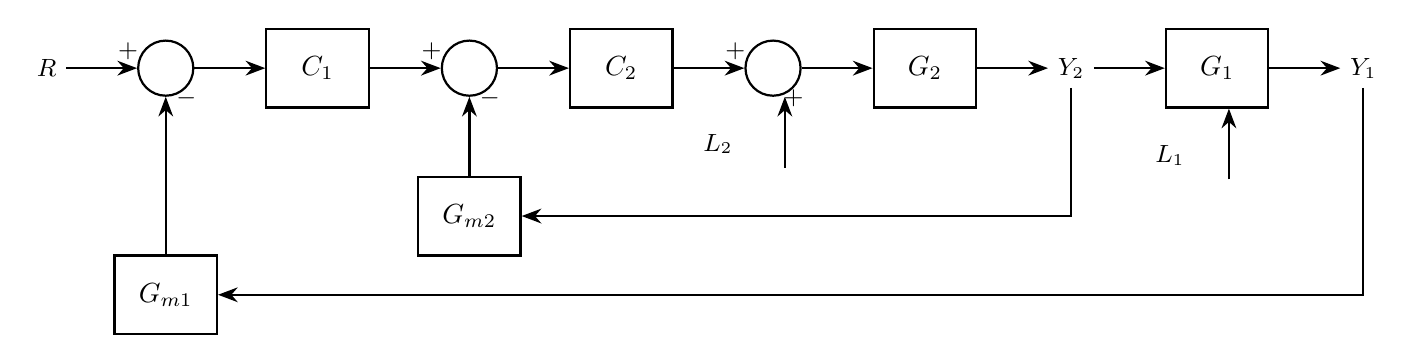
\begin{tikzpicture}[
  block/.style={draw=black, thick, minimum height=10mm, minimum width=13mm, inner sep=2pt},
  sum/.style={circle, draw=black, thick, minimum size=7mm, inner sep=0pt},
  sign/.style={font=\itshape\small},
  arr/.style={-{Stealth[length=2.5mm]}, thick},
  node distance=8mm and 9mm,
]
% caminho direto
\node[sign] (R) {$R$};
\node[sum, right=of R] (s1) {};
\node[sign] at ($(s1.center)+(-4.8mm,2.2mm)$) {$+$};
\node[sign] at ($(s1.center)+(2.6mm,-3.8mm)$) {$-$};
\node[block, right=of s1] (C1) {$C_1$};
\node[sum, right=of C1] (s2) {};
\node[sign] at ($(s2.center)+(-4.8mm,2.2mm)$) {$+$};
\node[sign] at ($(s2.center)+(2.6mm,-3.8mm)$) {$-$};
\node[block, right=of s2] (C2) {$C_2$};
\node[sum, right=of C2] (s3) {};
\node[sign] at ($(s3.center)+(-4.8mm,2.2mm)$) {$+$};
\node[sign] at ($(s3.center)+(2.6mm,-3.8mm)$) {$+$};
\node[block, right=of s3] (G2) {$G_2$};
\node[sign, right=of G2] (Y2) {$Y_2$};
\node[block, right=of Y2] (G1) {$G_1$};
\node[sign, right=of G1] (Y1) {$Y_1$};

% L2 entrando por baixo
\draw[arr] ($(s3.south)+(1.5mm,-9mm)$) -- ($(s3.south)+(1.5mm,0mm)$);
% L1 entrando por baixo em G1
\draw[arr] ($(G1.south)+(1.5mm,-9mm)$) -- ($(G1.south)+(1.5mm,0mm)$);
\node[sign] at ($(G1.south)+(-6mm,-6mm)$) {$L_1$};
\node[sign] at ($(s3.south)+(-7mm,-6mm)$) {$L_2$};

\draw[arr] (R) -- (s1);
\draw[arr] (s1) -- (C1);
\draw[arr] (C1) -- (s2);
\draw[arr] (s2) -- (C2);
\draw[arr] (C2) -- (s3);
\draw[arr] (s3) -- (G2);
\draw[arr] (G2) -- (Y2);
\draw[arr] (Y2) -- (G1);
\draw[arr] (G1) -- (Y1);

% realimentacao interna via Gm2
\node[block, below=10mm of s2] (Gm2) {$G_{m2}$};
\draw[arr] (Y2.south) |- (Gm2.east);
\draw[arr] (Gm2) -- (s2.south);
% realimentacao externa via Gm1
\node[block, below=20mm of s1] (Gm1) {$G_{m1}$};
\draw[arr] (Y1.south) |- (Gm1.east);
\draw[arr] (Gm1) -- (s1.south);
\end{tikzpicture}%
}
\end{document}
